\documentclass[hide notes,intlimits]{beamer}

\mode<presentation>
{
  \usetheme[footline]{PISMshade}
  \setbeamercovered{transparent}
}

% load packages
\usepackage{multimedia}
\usepackage[english]{babel}
\usepackage[latin1]{inputenc}
\usepackage[T1]{fontenc}
\usepackage{lmodern}
\usepackage{pdfpages}
\usepackage[multidot]{grffile}

%\setbeameroption{show notes on second screen=right}

\usepackage{tikz}
\usetikzlibrary{shapes,arrows}
\usetikzlibrary{shadows}

\definecolor{dark red}{HTML}{E41A1C}
\definecolor{dark green}{HTML}{4DAF4A}
\definecolor{dark violet}{HTML}{984EA3}
\definecolor{dark blue}{HTML}{084594}
\definecolor{dark orange}{HTML}{FF7F00}
\definecolor{light blue}{HTML}{377EB8}
\definecolor{light red}{HTML}{FB9A99}
\definecolor{light violet}{HTML}{CAB2D6}

\setbeamercolor{boxed}{fg=black,bg=light blue!25}
\graphicspath{{../figures_2018_08/}{figures/}}

\newenvironment{transbox}[1][]{%
\begin{tikzpicture}
\node[drop shadow,rounded corners,text width=.9\textwidth,fill=white, fill opacity=#1,text opacity=1] \bgroup
}{
\egroup;\end{tikzpicture}} 

\newenvironment{transbox-tight}{%
\begin{tikzpicture}
\node[drop shadow,rounded corners,fill=uaf yellow, fill opacity=0.75,text opacity=1] \bgroup
}{
\egroup;\end{tikzpicture}} 

\newcommand{\jl}{[\![}
\newcommand{\jr}{]\!\hskip 0.003cm ]}
\newcommand{\bpsi}{\boldsymbol{\psi}}
\newcommand{\bPsi}{\boldsymbol{\Psi}}
\newcommand{\bphi}{\boldsymbol{\phi}}
\newcommand{\bPhi}{\boldsymbol{\Phi}}
\newcommand{\bn}{\mathbf{n}}
\newcommand{\bq}{\mathbf{q}}
\newcommand{\bv}{\mathbf{v}}
\newcommand{\D}{\,\mathrm{d}}
\newcommand{\Tsnow}{T_{\text{snow}}}
\newcommand{\Hatm}{H_{\text l}^{\text{atm}}}

\newcommand{\mathtext}[1]{\mathsf{#1}}

% title page
\title[PISM] % (optional, use only with long paper titles)
{The Parallel Ice Sheet Model}
\subtitle{PISM}

\author[Aschwanden, Khroulev] % (optional, use only with lots of authors)
{A.~Aschwanden \& C.~Khroulev}
% - Give the names in the same order as the appear in the paper.
% - Use the \inst{?} command only if the authors have different
%   affiliation.

% - Use the \inst command only if there are several affiliations.
% - Keep it simple, no one is interested in your street address.

\titlegraphic{\vskip-1.cm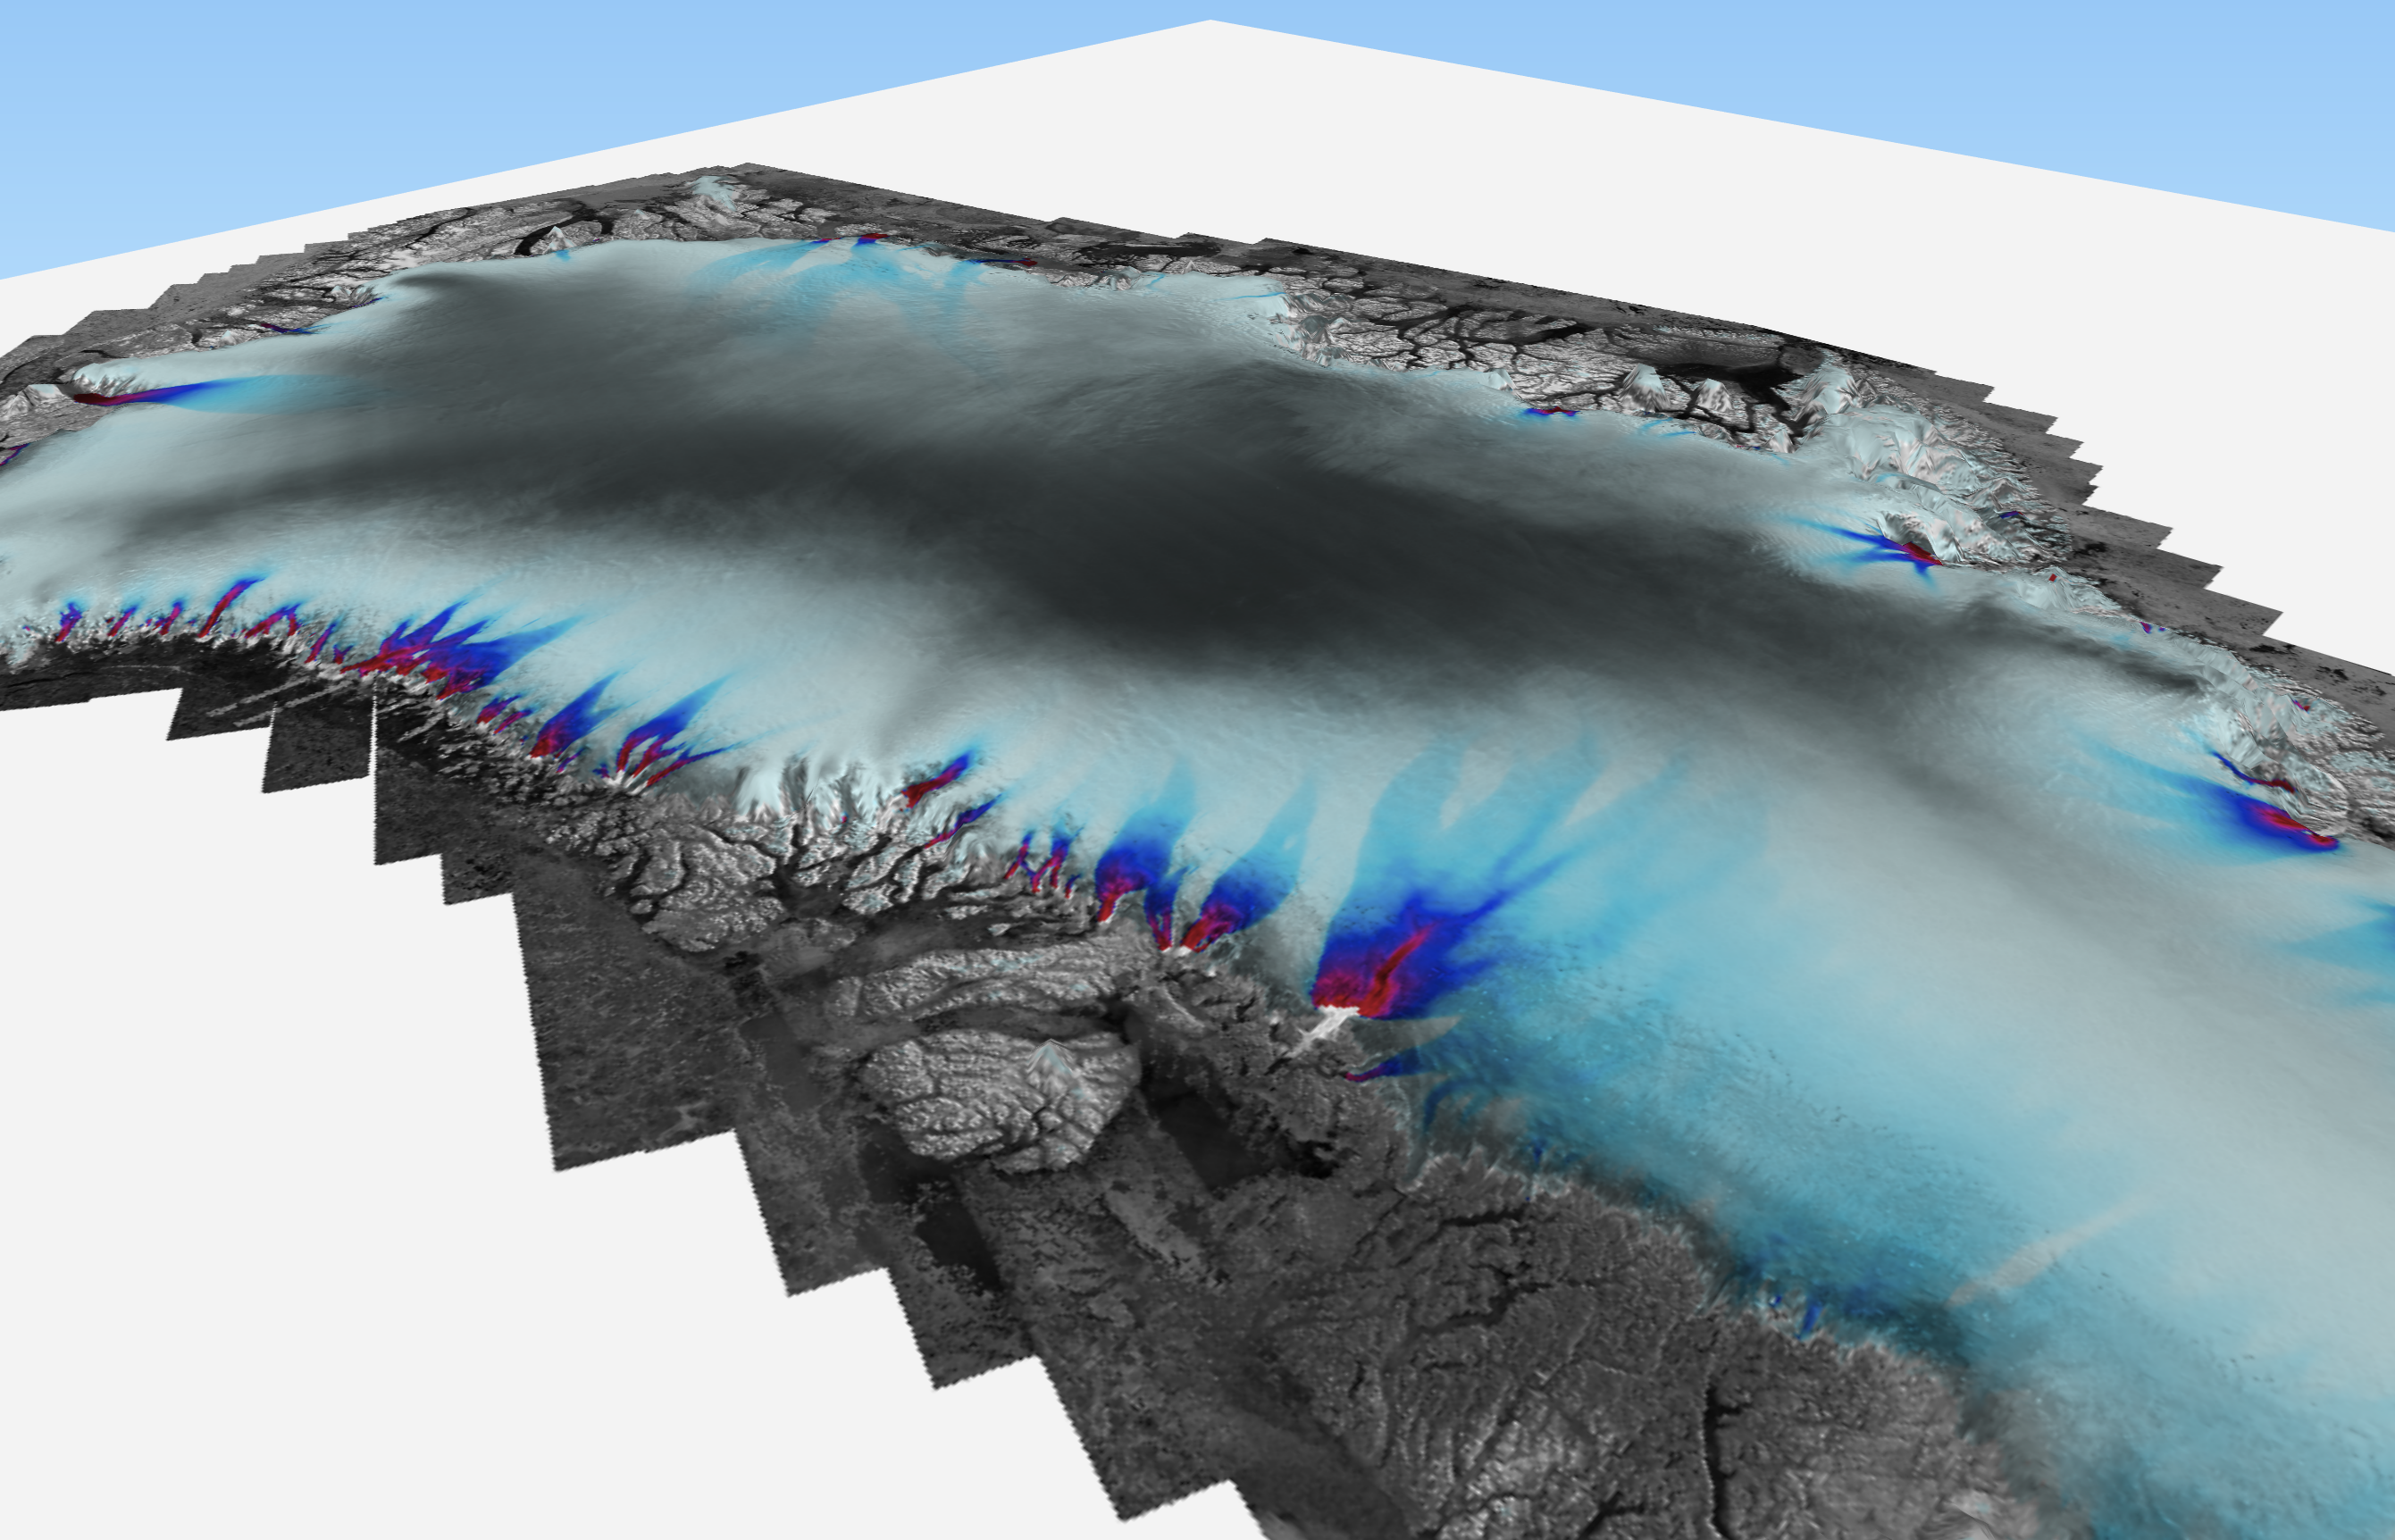
\includegraphics[height=4.5cm]{gris-flow-3d}}

\date{}


\subject{The Parallel Ice Sheet Model}

\begin{document}


\setbeamertemplate{background canvas}
  {
     \tikz{\node[inner sep=0pt,opacity=1.0] {\includegraphics[width=\paperwidth]{pism_beamer_shade_bg}};}
} 

% insert titlepage
\begin{frame}
  \titlepage
\end{frame}

\setbeamertemplate{background canvas}
  {
} 


\begin{frame}
  The Parallel Ice Sheet Model PISM v1.0 is open source and capable of high resolution. It has been widely adopted as a tool for doing science.
  
  Features include:

  \begin{itemize}
  \item extensible atmospheric/ocean coupling
  \item complete documentation
  \item parallel simulations using MPI \& PETSc
  \item reads and writes CF-compliant NetCDF
  \item inversion toolbox in Python
  \item verification and validation tools
  \end{itemize}
  
\end{frame}


\begin{frame}{Strengths}
  \begin{itemize}
  \item tried-and-true, widely adopted by the community
    \item computationally efficient:
      \begin{itemize}
      \item high-resolutions simulations over long time scales
      \end{itemize}
    \item flexibility
      \begin{itemize}
      \item can handle a variety of environnmental forcings
      \end{itemize}
      \item comprehensive user documentation
      \item adheres to community standards 
    \end{itemize}
\end{frame}


\begin{frame}{Brief History}

  
  \begin{columns}[c]
    \begin{column}{.1\linewidth}
      before 2001
    \end{column}
    \begin{column}{.1\linewidth}
      \begin{figure}
        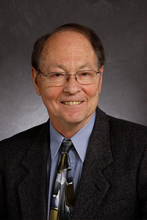
\includegraphics[width=\textwidth]{craig_lingle}
      \end{figure}
    \end{column}
    \begin{column}{.55\linewidth}
      \begin{itemize}
      \item Orographic Precipitation
      \item Erosion
      \end{itemize}
    \end{column}
  \end{columns}  
  \begin{columns}
    \begin{column}{.1\linewidth}
      before 2001
    \end{column}
    \begin{column}{.1\linewidth}
      \begin{figure}
        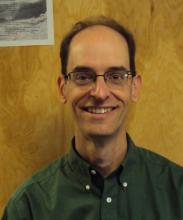
\includegraphics[width=\textwidth]{ed_bueler}
      \end{figure}
    \end{column}
    \begin{column}{.55\linewidth}
      \begin{itemize}
      \item Orographic Precipitation
      \item Erosion
      \end{itemize}
    \end{column}
  \end{columns}  
  \begin{columns}
    \begin{column}{.1\linewidth}
      before 2001
    \end{column}
    \begin{column}{.1\linewidth}
      \begin{figure}
        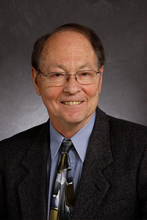
\includegraphics[width=\textwidth]{craig_lingle}
      \end{figure}
    \end{column}
    \begin{column}{.55\linewidth}
      \begin{itemize}
      \item Orographic Precipitation
      \item Erosion
      \end{itemize}
    \end{column}
  \end{columns}  

\end{frame}

\begin{frame}{Applications}
  \begin{figure}
    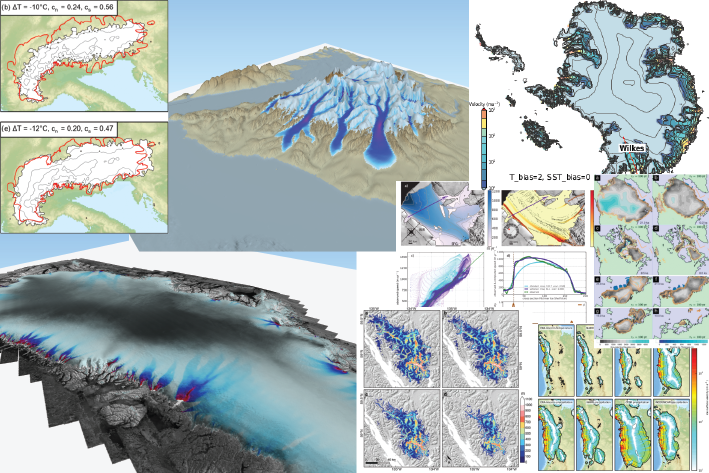
\includegraphics[width=\textwidth]{pism-applications-composite-01}
  \end{figure}

\end{frame}


\begin{frame}{Olympics Peninsula}
    \begin{columns}[c]
      \begin{column}{.45\linewidth}
        \begin{figure}
          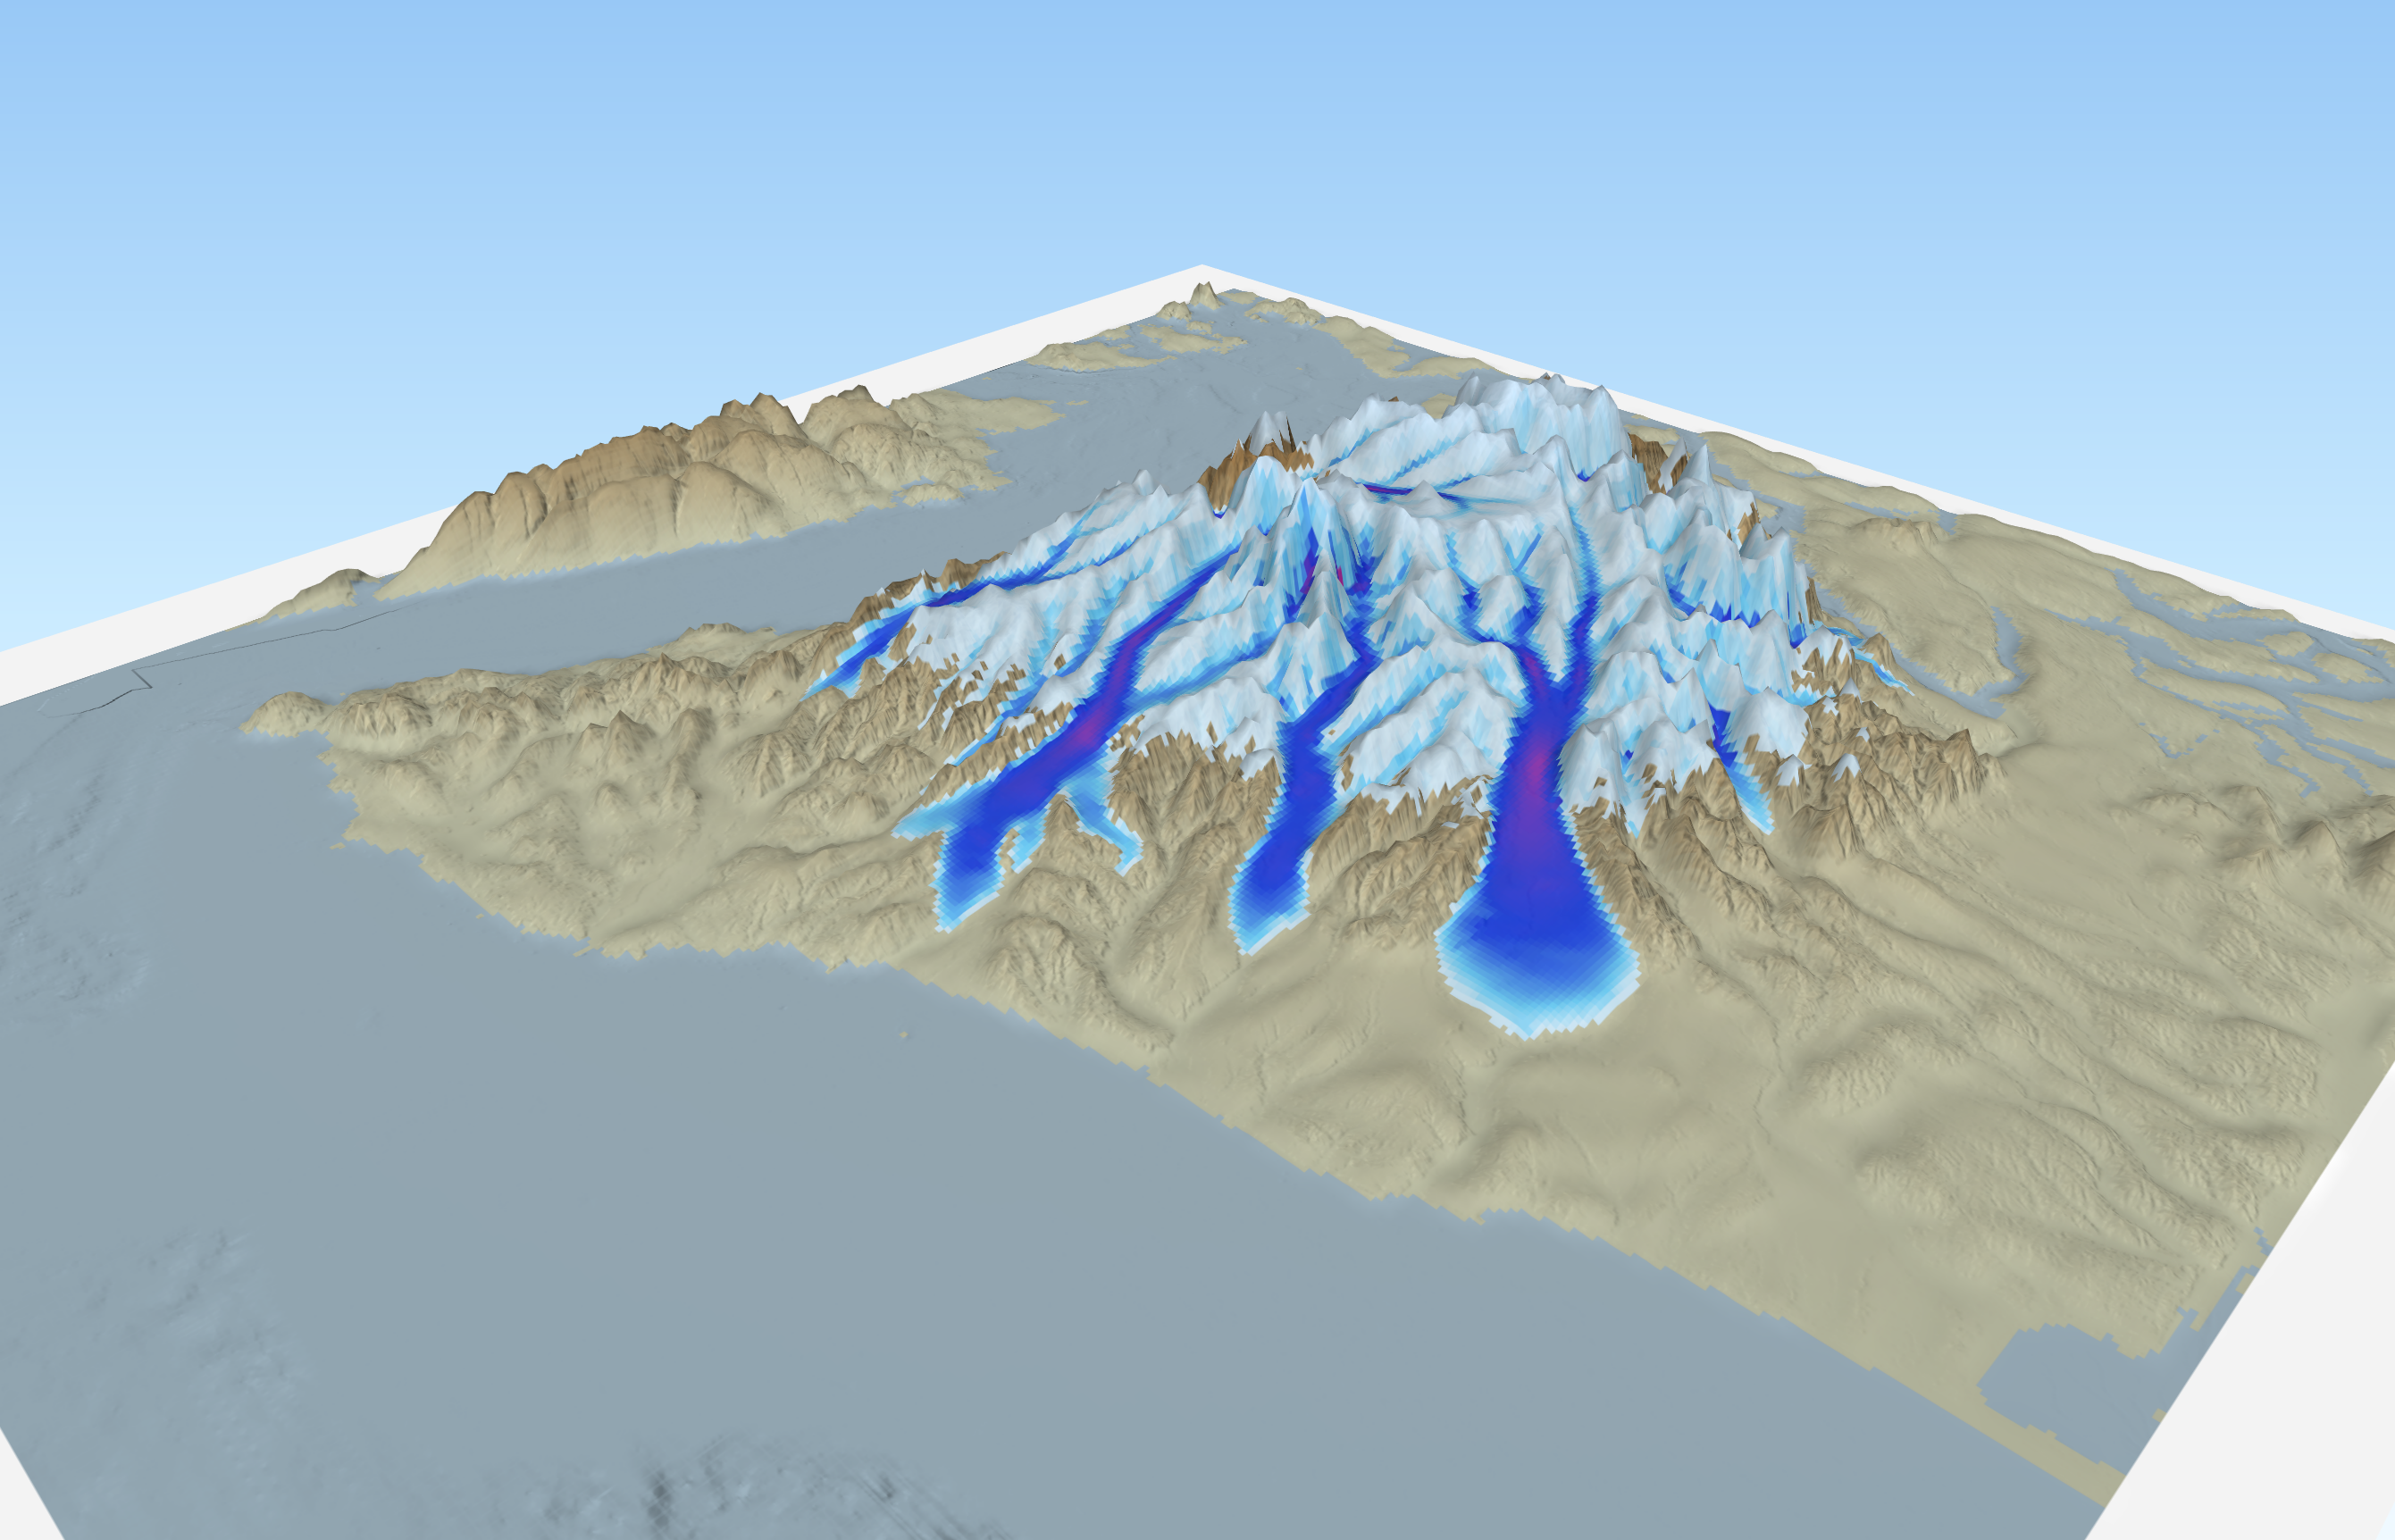
\includegraphics[width=\textwidth]{olympics-3d}
        \end{figure}
      \end{column}
      \begin{column}{.55\linewidth}
        \begin{itemize}
        \item Orographic Precipitation
        \item Erosion
        \end{itemize}
      \end{column}
    \end{columns}  
\end{frame}


\begin{frame}{PICO}
    \begin{columns}[c]
      \begin{column}{.45\linewidth}
        \begin{figure}
          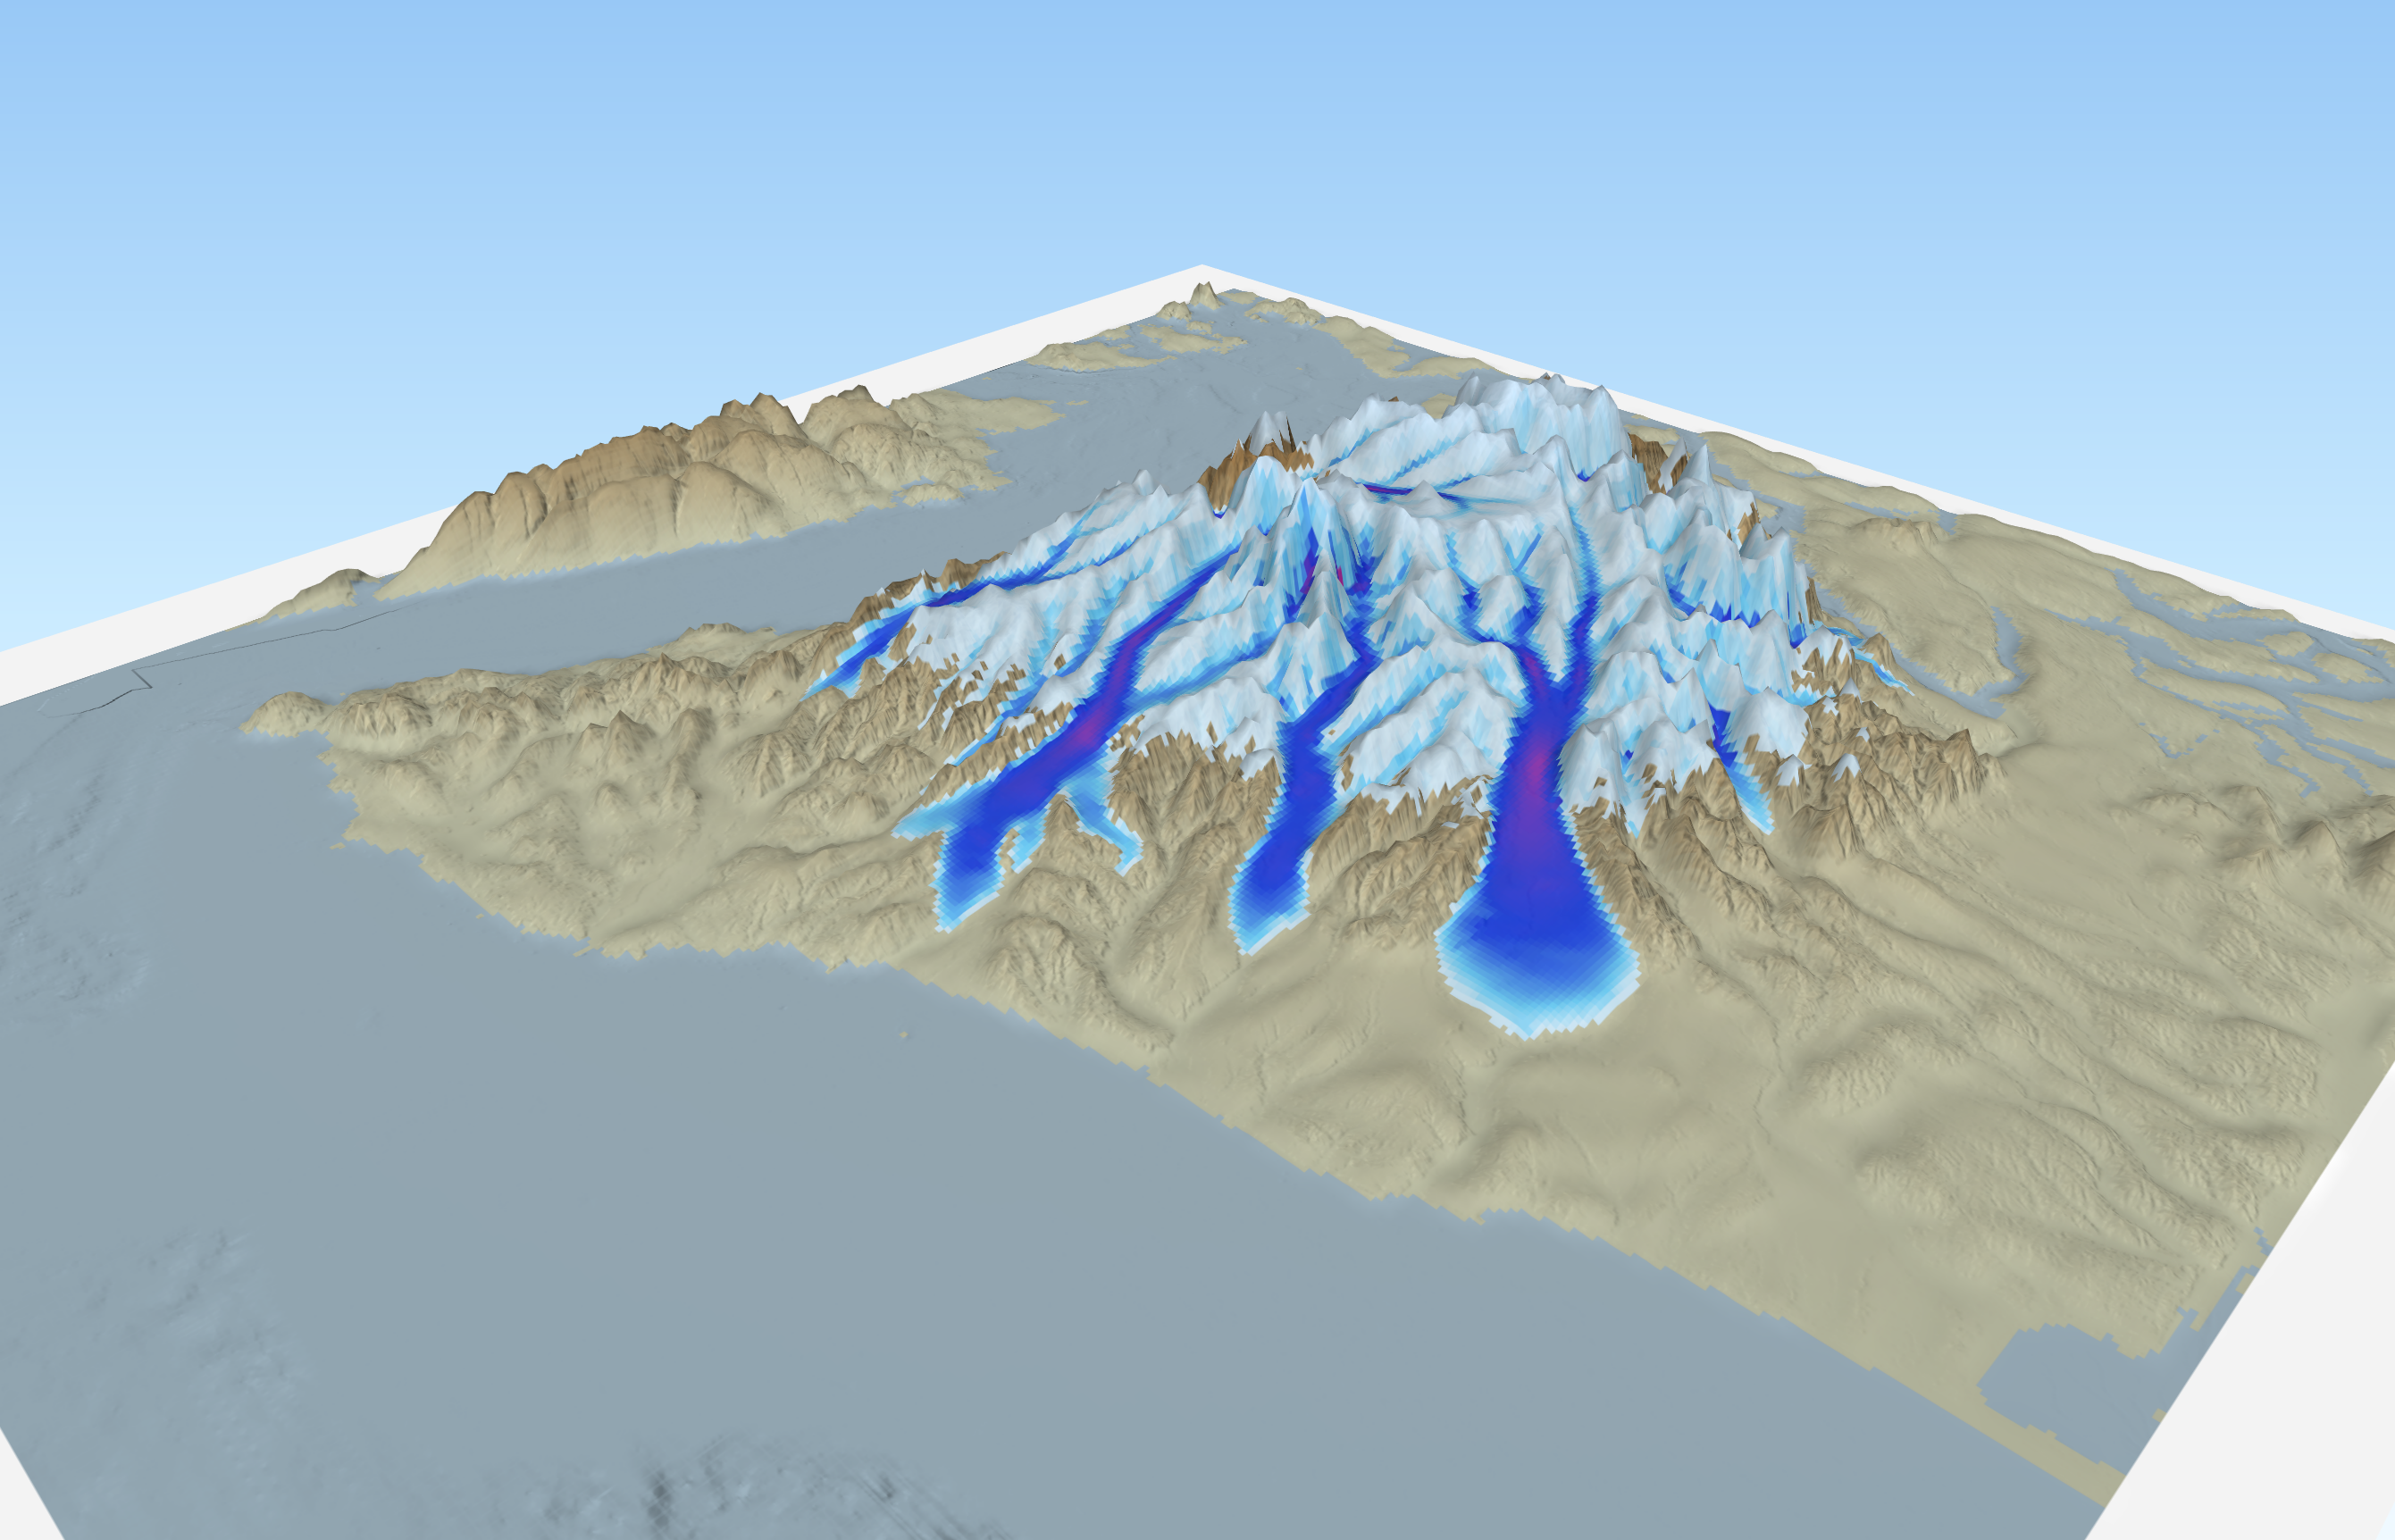
\includegraphics[width=\textwidth]{olympics-3d}
        \end{figure}
      \end{column}
      \begin{column}{.55\linewidth}
        \begin{itemize}
        \item Orographic Precipitation
        \item Erosion
        \end{itemize}
      \end{column}
    \end{columns}  
\end{frame}


\begin{frame}{Greenland}
    \begin{columns}[c]
      \begin{column}{.45\linewidth}
        \begin{figure}
          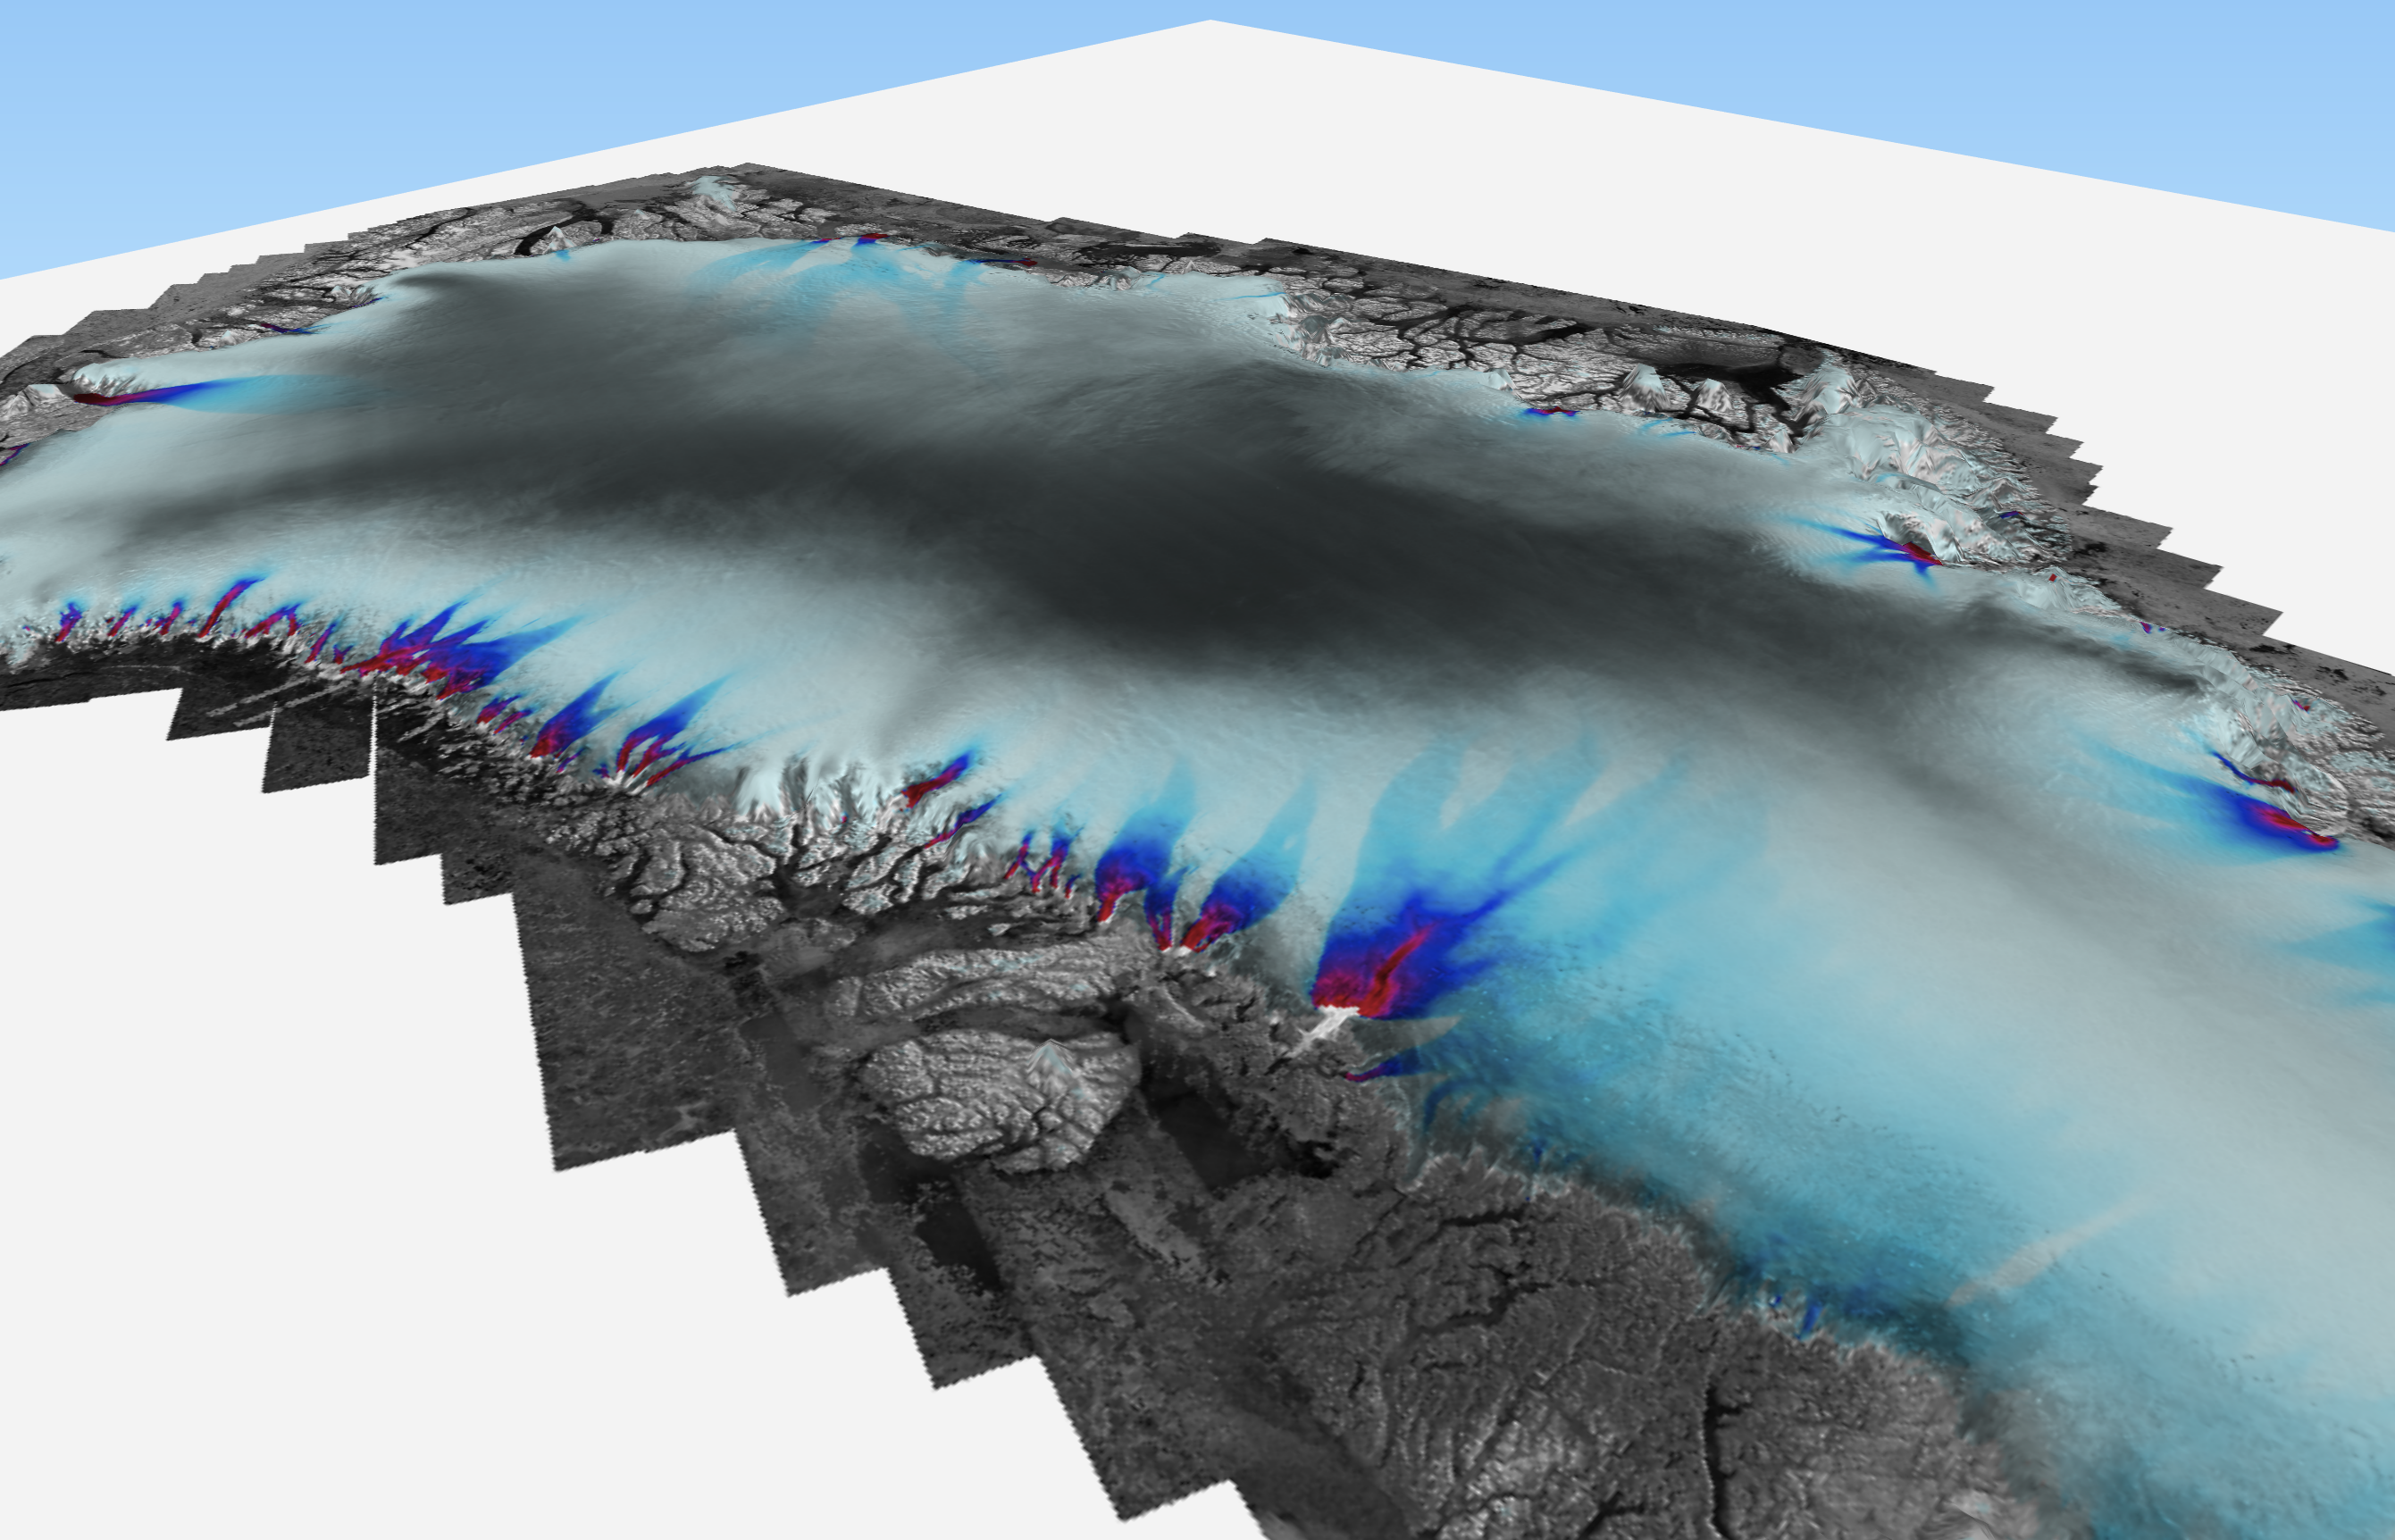
\includegraphics[width=\textwidth]{gris-flow-3d}
        \end{figure}
      \end{column}
      \begin{column}{.55\linewidth}
        \begin{itemize}
        \item Outlet Glacier Resolving
        \item Uncertainty Quantification
        \end{itemize}
      \end{column}
    \end{columns}
\end{frame}

\end{document}